
\begin{frame}\frametitle{Physics objects puzzle}
\centering\myskip

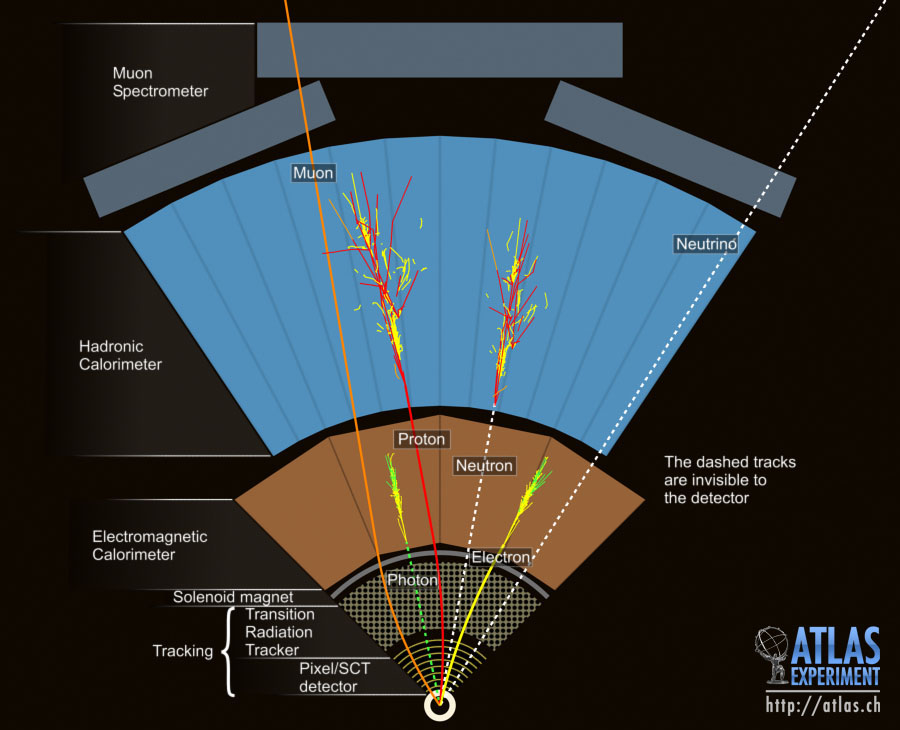
\includegraphics[height=0.85\textheight, width=1.\textwidth]{../detector/figures/detection}

\end{frame}



\begin{frame}\frametitle{One lepton}
\footnotesize\centering

\begin{minipage}{.5\textwidth}\centering
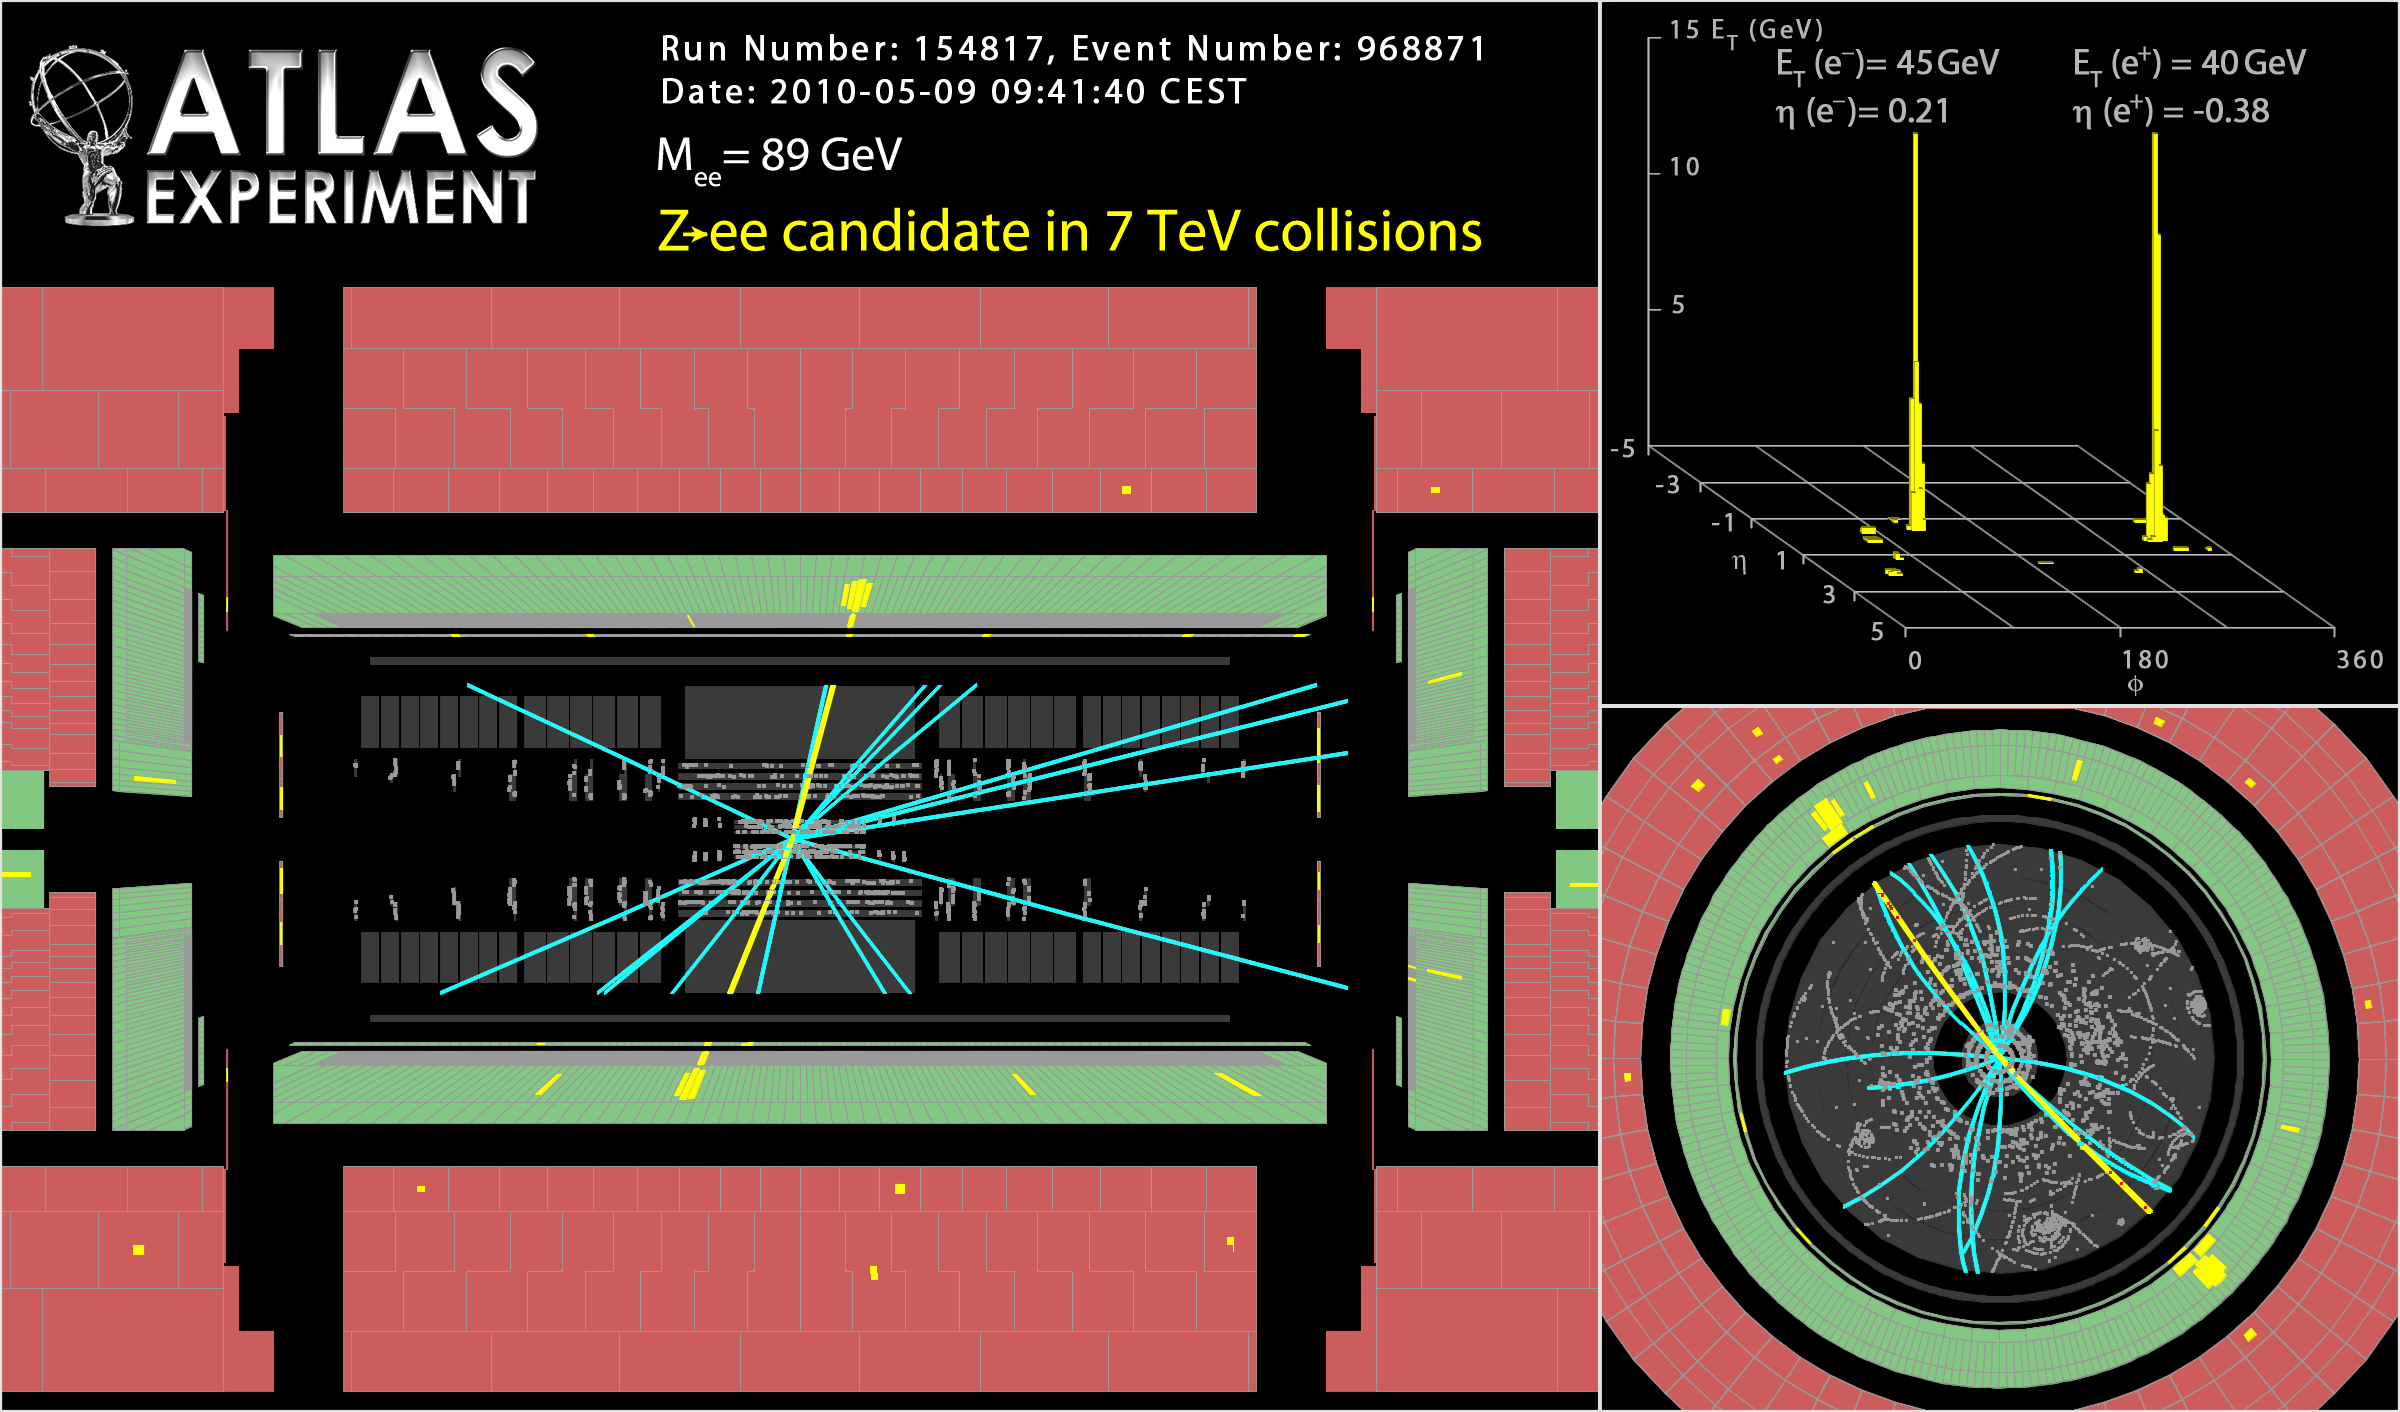
\includegraphics[width=.9\textwidth,height=0.3\textheight]{pics/Zee}

\begin{itemize}
\item $|\eta|<2.47$ ID track $\leftrightarrow$ EM deposit
\item $E_{\rm calo}$ consistent with $p_{\rm T, ID}$
\item calibrated with $Z\to ee$ events
\end{itemize}
{\cccolor \bfseries +}\\
\begin{itemize}
\item excluded $1.37< |\eta|< 1.52$
%\item $\et = E_{\rm cluster}/\cosh\eta_{\rm track} > 25\gev$, $|z_0|<2~$mm.
\item $\et > 25\gev$, $|z_0|<2~$mm
\item isolation cuts {\scriptsize\texttt{EtCone20}, \texttt{PtCone30}}
\item electron-jet overlap removal
\item {\scriptsize\texttt{EF\_e24vhi\_medium1} $||$ \texttt{EF\_e60\_medium1}}
\end{itemize}


\end{minipage}\begin{minipage}{.5\textwidth}\centering


\begin{itemize}
\item \texttt{Muid}: MS track $\leftrightarrow$ ID track ($|\eta|<2.47$)
\item $p_{\rm T,MS}$ corrected for mip loss
\item $p_{\rm T}$ weighted average MS $\leftrightarrow$ ID
\item calibrated with $Z\to \mu\mu$ events
\end{itemize}
{\cccolor \bfseries +}\\
\begin{itemize}
\item $\pt > 25\gev$, $|z_0|<2~$mm
\item isolation cut \texttt{PtCone20}
\item mini-isolation cut
\item \texttt{EF\_mu24i\_tight} $||$ \texttt{EF\_mu36\_tight}
\end{itemize}

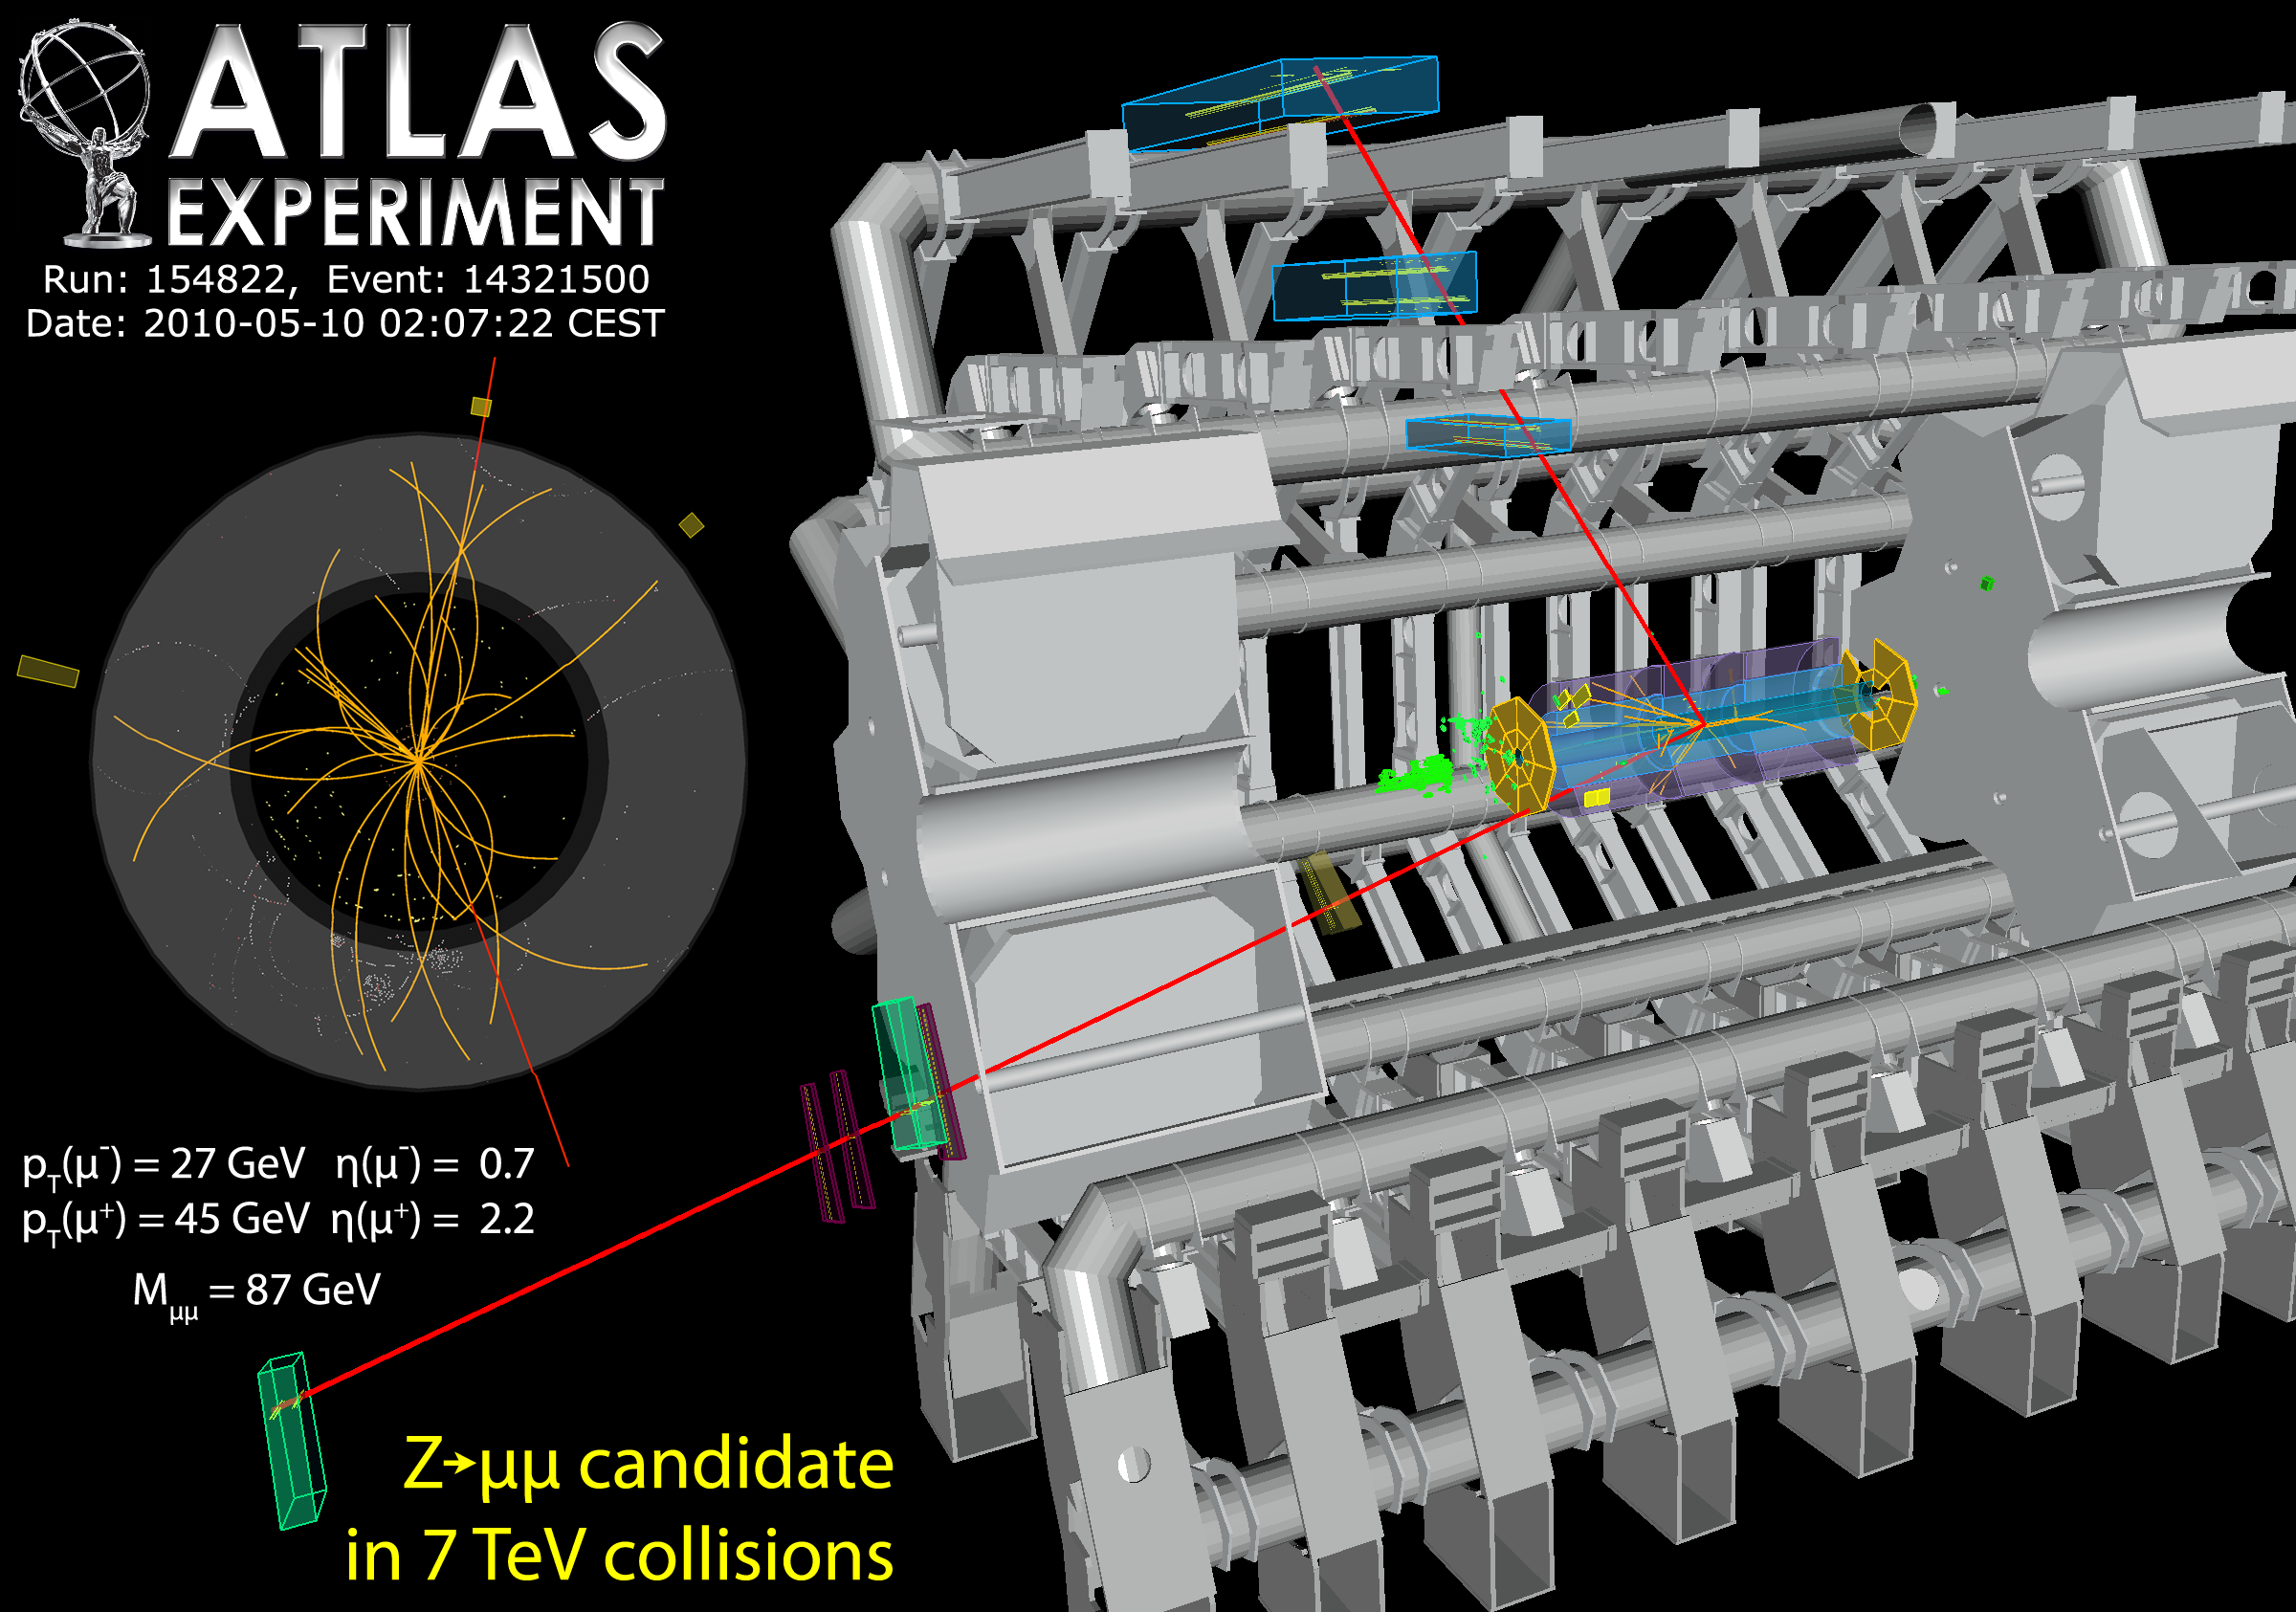
\includegraphics[width=.78\textwidth,height=0.3\textheight]{pics/Zmumu}

\end{minipage}


\end{frame}



\begin{frame}\frametitle{Many jets}
\centering\footnotesize

\begin{minipage}{.5\textwidth}\centering

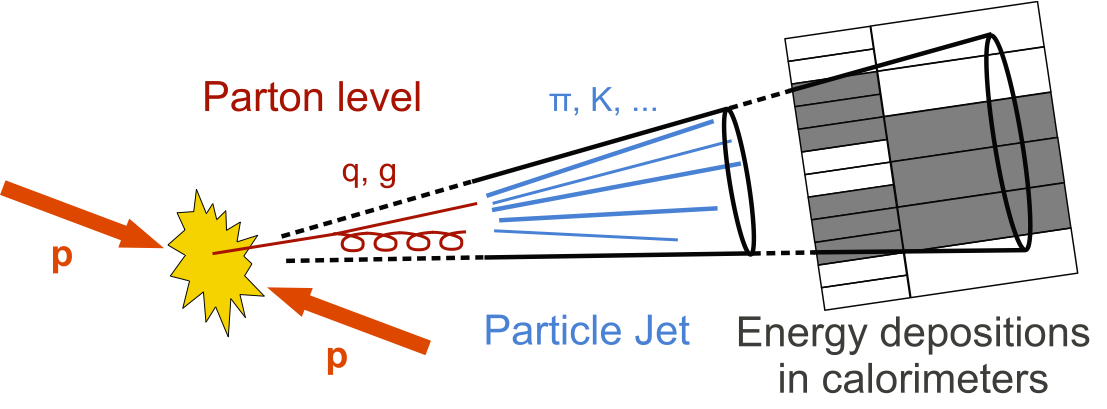
\includegraphics[width=.78\textwidth]{pics/Sketch_PartonParticleCaloJet.png}\\
%\resizebox{1.\textwidth}{!}{from \url{http://cms.web.cern.ch/news/jets-cms-and-determination-their-energy-scale}}

\begin{itemize}
\item Combine calorimeter clusters using anti-$k_t$ algorithm with $R=0.4$
\end{itemize}
$d_{ij}=min(\dfrac{1}{k_{t_i}^{2}},\dfrac{1}{k_{t_j}^{2}})\frac{\Delta R_{ij}^{2}}{R^{2}}$
\begin{itemize}
\item LC clusters energy
\item Pile-up and JES correction
\end{itemize}
{\cccolor \bfseries +}\\
\begin{itemize}
\item $\pt>25\gev$, $|\eta|<2.5$
\item JVF$>0.5$
\item jet-electron overlap removal
\end{itemize}


\end{minipage}\begin{minipage}{.5\textwidth}\centering

\vskip-5ex
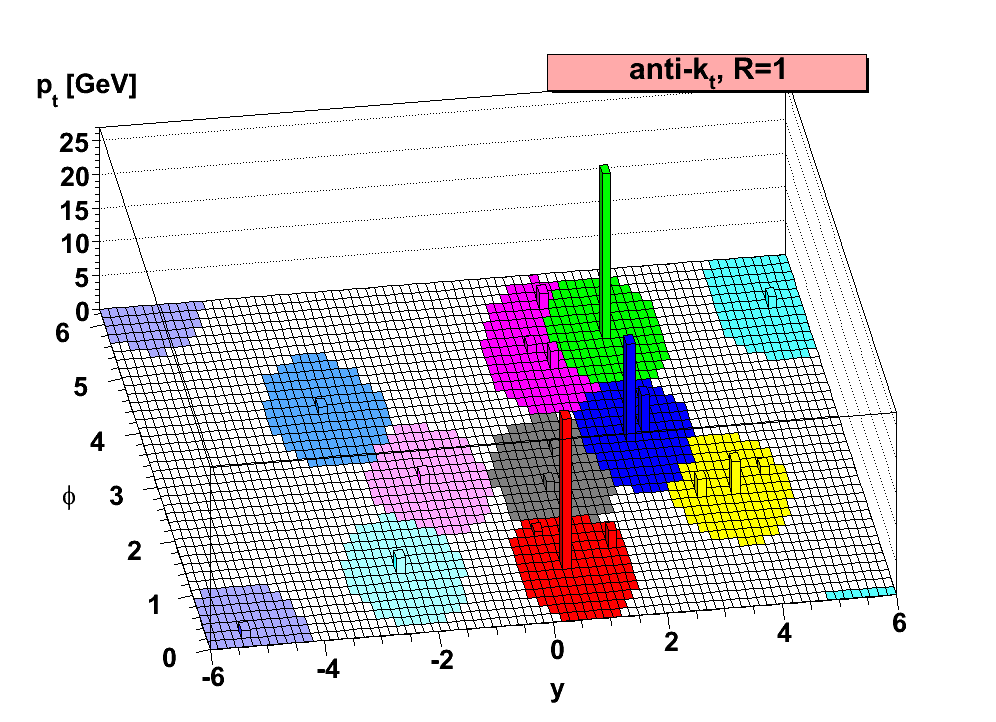
\includegraphics[width=.8\textwidth]{pics/antikt}\\
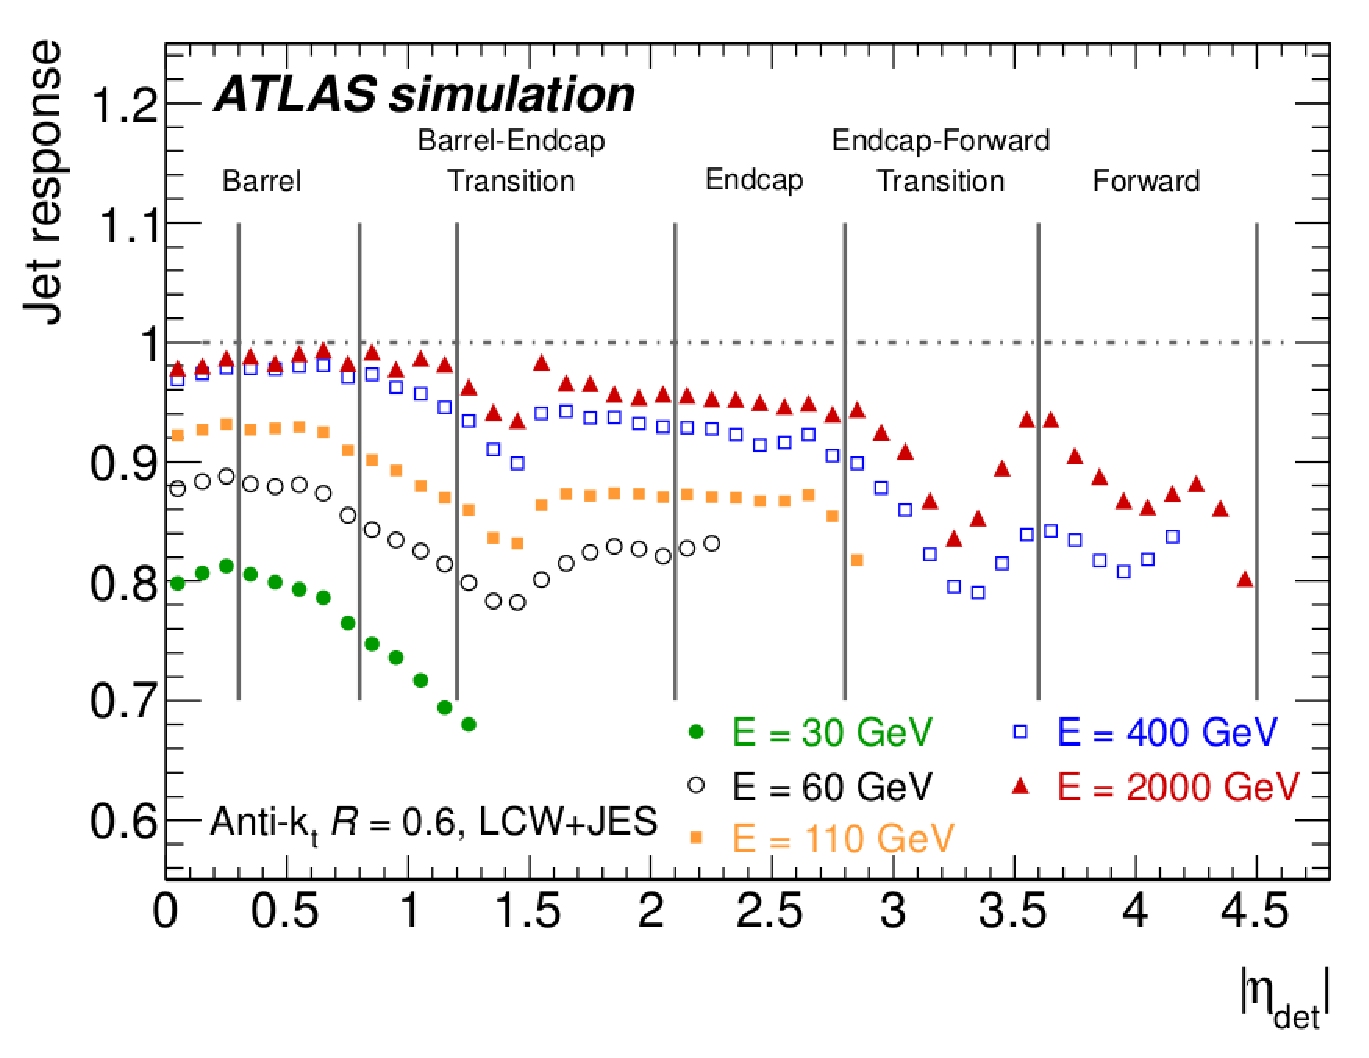
\includegraphics[width=.9\textwidth]{pics/corr_jet_lcw}

\end{minipage}


\end{frame}



\begin{frame}\frametitle{\btag ging}
\centering\footnotesize

\begin{minipage}{.3\textwidth}\centering

$b$ quark $\Rightarrow$ $B$ hadron ($\lambda\sim 10^{-12}$~s)\\
{\large$\Downarrow$}\\
travels about 3~mm\\ before decaying

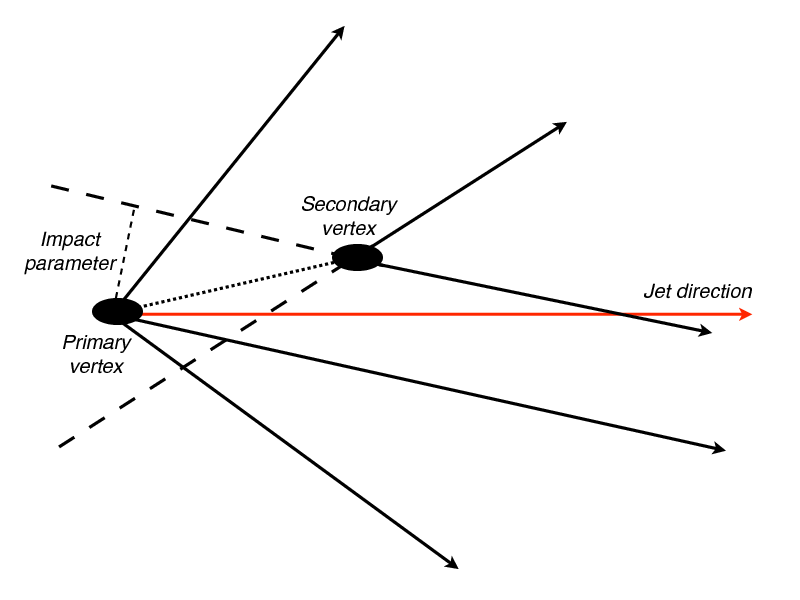
\includegraphics[width=.8\textwidth]{../objectsreconstruction/figures/Picture-b-tagging-2.png}

\end{minipage}\begin{minipage}{.7\textwidth}\centering

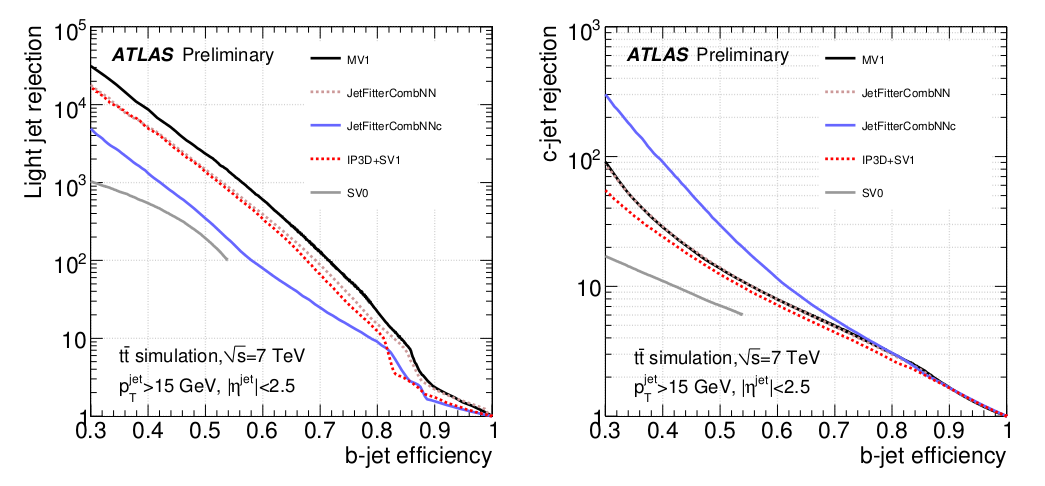
\includegraphics[width=1.\textwidth]{../objectsreconstruction/figures/btageffs.png}

\end{minipage}

\myskip

\begin{minipage}{.4\textwidth}\centering


various algorithms exploit ID track info to identify \bjet s

\begin{itemize}
\item \texttt{\cccolor MV1} algorithm @ 70\% efficiency, $\sim 130$ rejection
\end{itemize}

\end{minipage}\begin{minipage}{.6\textwidth}\centering

Events are selected through \\a cut on the \btag-weight computed\\
{\large$\Downarrow$}\\
with 70\% efficiency, high multiplicities will suffer

\begin{itemize}
\item {\cccolor TagRateFunction} method
\end{itemize}


\end{minipage}


\end{frame}



\begin{frame}\frametitle{Missing transverse energy}
\centering\myskip

\begin{minipage}{.5\textwidth}\centering

\includegraphics[width=.9\textwidth]{pics/real_et}\\
{\tiny from \url{http://tomwhyntie.wordpress.com/research/}}

\end{minipage}\begin{minipage}{.5\textwidth}\centering
\end{minipage}
$$\begin{array}{lcl}
%E^{\rm miss}_{x,y} & = & E^{\rm RefEle}_{x,y} + E^{\rm RefGamma}_{x,y} + E^{\rm RefJet}_{x,y} + E^{\rm RefMuon}_{x,y} + E^{\rm SoftJet}_{x,y} + E^{\rm CellOut}_{x,y}\\
E^{\rm miss}_{T} & = & \big|-\sum\vec{p}_T \big| = \sqrt{(E^{\rm miss}_{x})^2 + (E^{\rm miss}_{y})^2} ,\\
E^{\rm miss}_{x} & = & -\sum\vec{p}_x ,\\
E^{\rm miss}_{y} & = & -\sum\vec{p}_y ,\\
\end{array}$$


\end{frame}

